% ======================================================================
% HHDMS — 10-minute semi-technical presentation
% Compile: pdflatex hhdms_slides.tex  (run twice for footline refs)
% ======================================================================
\documentclass[aspectratio=169,11pt]{beamer}

\usepackage[T1]{fontenc}
\usepackage{lmodern}
\usepackage{tikz}
\usetikzlibrary{arrows.meta,positioning,calc,shapes.geometric}
\usepackage{booktabs}

% ---------- Brand colors ----------
\definecolor{TechTeal}{HTML}{00D4B2}      % bright accent (graphics)
\definecolor{TealDark}{HTML}{00806E}      % readable teal (text accents)
\definecolor{ClinicalNavy}{HTML}{0A2540}  % primary text / titles
\definecolor{SoftGray}{HTML}{F2F5F7}      % panel backgrounds
\definecolor{MidGray}{HTML}{8A9BA8}       % secondary text

% ---------- Beamer look ----------
\usetheme{default}
\setbeamercolor{normal text}{fg=ClinicalNavy,bg=white}
\setbeamercolor{structure}{fg=TealDark}
\setbeamercolor{frametitle}{fg=ClinicalNavy}
\setbeamercolor{title}{fg=ClinicalNavy}
\setbeamercolor{itemize item}{fg=TealDark}
\setbeamercolor{itemize subitem}{fg=TealDark}
\setbeamercolor{block title}{fg=white,bg=TealDark}
\setbeamercolor{block body}{fg=ClinicalNavy,bg=SoftGray}
\setbeamertemplate{itemize item}{\textcolor{TealDark}{\raisebox{1.2pt}{\rule{5pt}{5pt}}}}
\setbeamertemplate{navigation symbols}{}
\setbeamersize{text margin left=1.1em,text margin right=1.1em}

% Frametitle with teal underline bar
\setbeamertemplate{frametitle}{%
  \vskip0.8em%
  {\usebeamerfont{frametitle}\textbf{\insertframetitle}}\par%
  \vskip0.25em%
  {\color{TechTeal}\rule{2.6cm}{2.5pt}}\par%
  \vskip0.4em%
}

% Footline: short title | slide number
\setbeamertemplate{footline}{%
  \hbox{\begin{beamercolorbox}[wd=\paperwidth,ht=2.4ex,dp=1ex,leftskip=1.2em,rightskip=1.2em]{normal text}%
    {\scriptsize\color{MidGray}\insertshorttitle}\hfill{\scriptsize\color{MidGray}\insertframenumber\,/\,\inserttotalframenumber}%
  \end{beamercolorbox}}%
}

% ---------- Helper: dashed demo placeholder frame ----------
% \demoFrame{width}{height}{caption}
\newcommand{\demoFrame}[3]{%
  \begin{tikzpicture}[baseline=(current bounding box.center)]
    \draw[dashed,very thick,MidGray,rounded corners=4pt]
      (0,0) rectangle (#1,#2);
    \node at (#1/2,#2*0.58) {\color{MidGray}\large Screenshot};
    \node at (#1/2,#2*0.42) {\color{MidGray}\small (paste image here)};
    \node[anchor=north] at (#1/2,-0.12)
      {\parbox{#1}{\centering\color{TealDark}\footnotesize\textbf{#3}}};
  \end{tikzpicture}%
}

% ---------- Title metadata ----------
\title[HHDMS -- Home Healthcare Platform]{HHDMS}
\subtitle{Home Healthcare \& Diagnostic Center Management System\\
{\normalsize\itshape ``Home Healthcare, One Call Away''}}
\author[CSE 299 $\cdot$ NSU]{CSE 299 --- North South University\\[2pt]
{\small Team:\; Name 1 \and Name 2 \and Name 3 \and Name 4}}
\date{August 2026}

\begin{document}

% ======================================================================
\begin{frame}[plain]
  \titlepage
\end{frame}

% ======================================================================
\begin{frame}{The Problem \& Our Solution}
  \begin{columns}[T]
    \column{0.48\textwidth}
    \begin{block}{The Problem}
      \begin{itemize}
        \item Home healthcare in Bangladesh runs on phone calls --- no tracking, no records, no accountability
        \item Families cannot see where the doctor or nurse is
        \item Prescriptions and reports are paper-only, easily lost
        \item Payments are informal; billing is opaque
      \end{itemize}
    \end{block}
    \column{0.48\textwidth}
    \begin{block}{Our Solution: One Platform}
      \begin{itemize}
        \item A single call center books any service --- doctor visit, nursing, diagnostics, nutrition
        \item Patients watch their provider arrive in real time on a map
        \item Digital records: e-prescriptions, reports, invoices
        \item Secure online payments and instant notifications
      \end{itemize}
    \end{block}
  \end{columns}
  \vfill
  \centering
  {\footnotesize\itshape\color{TealDark} From an inbound phone call to a delivered home visit --- fully digital.}
\end{frame}

% ======================================================================
\begin{frame}{How It Works --- The Core Journey}
  \centering
  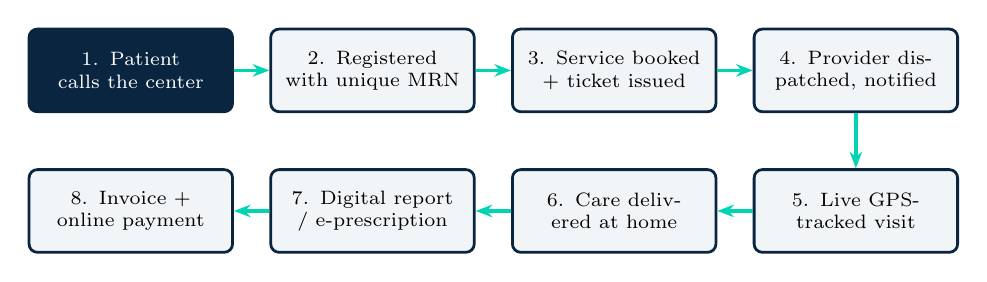
\begin{tikzpicture}[
      node distance=0.55cm and 0.45cm,
      jstep/.style={draw=ClinicalNavy,line width=1pt,rounded corners=3pt,
                    fill=SoftGray,text width=2.35cm,align=center,
                    minimum height=1.05cm,font=\scriptsize},
      arr/.style={-{Stealth[length=6pt]},line width=1.2pt,TechTeal},
    ]
    \node[jstep,fill=ClinicalNavy,text=white] (call) {1. Patient calls the center};
    \node[jstep,right=of call] (reg)   {2. Registered with unique MRN};
    \node[jstep,right=of reg]   (book) {3. Service booked + ticket issued};
    \node[jstep,right=of book]  (disp) {4. Provider dispatched, notified};
    \node[jstep,below=0.7cm of disp] (track) {5. Live GPS-tracked visit};
    \node[jstep,left=of track]  (serve) {6. Care delivered at home};
    \node[jstep,left=of serve]  (report){7. Digital report / e-prescription};
    \node[jstep,left=of report] (pay)   {8. Invoice + online payment};

    \draw[arr] (call) -- (reg);
    \draw[arr] (reg)  -- (book);
    \draw[arr] (book) -- (disp);
    \draw[arr] (disp) -- (track);
    \draw[arr] (track) -- (serve);
    \draw[arr] (serve) -- (report);
    \draw[arr] (report) -- (pay);
  \end{tikzpicture}

  \vspace{0.5cm}
  {\small Every step is timestamped and visible to the right people ---\\
   patient, provider, and operations staff.}
\end{frame}

% ======================================================================
\begin{frame}{System at a Glance}
  \centering
  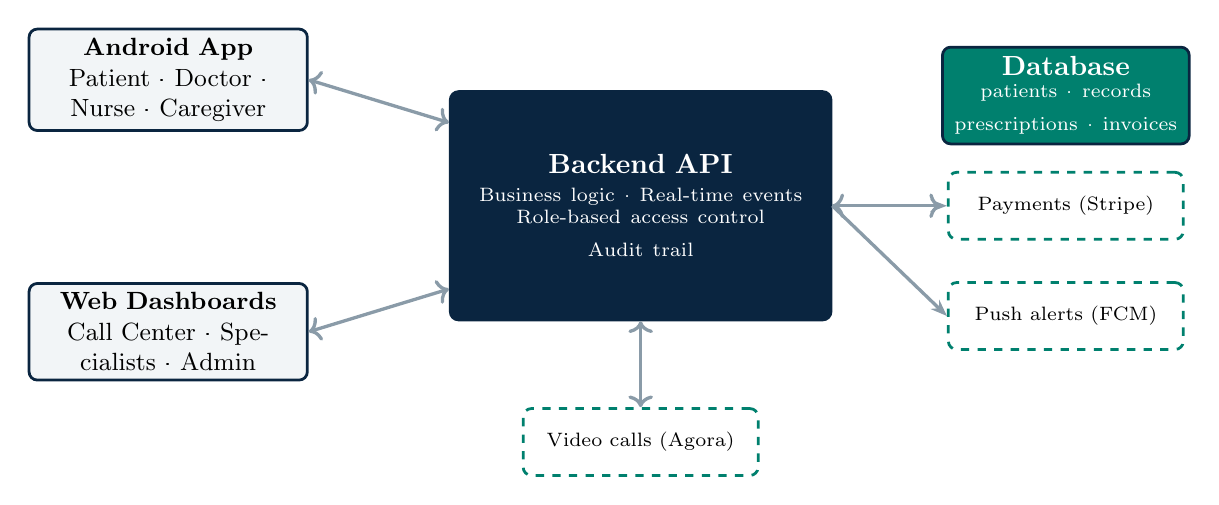
\begin{tikzpicture}[
      box/.style={draw=ClinicalNavy,line width=1pt,rounded corners=3pt,
                  align=center,minimum height=1.15cm},
      client/.style={box,fill=SoftGray,text width=3.3cm,font=\small},
      core/.style={box,fill=ClinicalNavy,text=white,text width=4.6cm,minimum height=2.9cm},
      integ/.style={draw=TealDark,line width=1pt,dashed,rounded corners=3pt,
                    fill=white,text width=2.75cm,align=center,
                    minimum height=0.85cm,font=\scriptsize},
      arr/.style={-{Stealth[length=6pt]},line width=1.2pt,MidGray},
    ]
    % Clients
    \node[client] (android) at (0,1.6)  {\textbf{Android App}\\ Patient · Doctor · Nurse · Caregiver};
    \node[client] (web)     at (0,-1.6) {\textbf{Web Dashboards}\\ Call Center · Specialists · Admin};
    % Core
    \node[core] (api) at (6,0) {\textbf{Backend API}\\[2pt]
        \scriptsize Business logic · Real-time events\\ \scriptsize Role-based access control\\ \scriptsize Audit trail};
    % Data
    \node[box,fill=TealDark,text=white,text width=2.9cm] (db) at (11.4,1.4)
        {\textbf{Database}\\ \scriptsize patients · records\\ \scriptsize prescriptions · invoices};
    \node[integ] (stripe) at (11.4,0)   {Payments (Stripe)};
    \node[integ] (fcm)    at (11.4,-1.4){Push alerts (FCM)};
    \node[integ] (agora)  at (6,-3.0)   {Video calls (Agora)};

    \draw[arr,<->] (android.east) -- ($(api.north west)!0.28!(api.west)$);
    \draw[arr,<->] (web.east) -- ($(api.south west)!0.28!(api.west)$);
    \draw[arr,<->] (api.east) -- (db.west |- api.east -| db.west);
    \draw[arr] (api.east) -- (stripe.west);
    \draw[arr] (api.east) -- (fcm.west);
    \draw[arr,<->] (api.south) -- (agora.north);
  \end{tikzpicture}
\end{frame}

% ======================================================================
\begin{frame}{One Platform, Nine Roles}
  \centering
  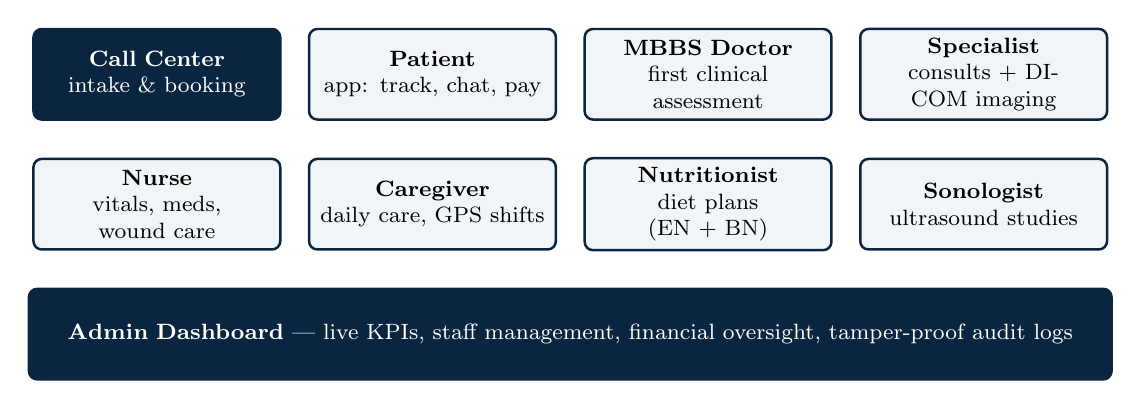
\begin{tikzpicture}[
      role/.style={draw=ClinicalNavy,line width=0.9pt,rounded corners=3pt,
                   fill=SoftGray,text width=2.9cm,align=center,
                   minimum height=1.15cm,font=\footnotesize},
      hl/.style={role,fill=ClinicalNavy,text=white},
    ]
    \node[hl]  (cc) at (0,0)     {\textbf{Call Center}\\ intake \& booking};
    \node[role](pat) at (3.5,0)  {\textbf{Patient}\\ app: track, chat, pay};
    \node[role](mbbs)at (7.0,0)  {\textbf{MBBS Doctor}\\ first clinical assessment};
    \node[role](spec)at (10.5,0) {\textbf{Specialist}\\ consults + DICOM imaging};

    \node[role](nurse)at (0,-1.65) {\textbf{Nurse}\\ vitals, meds, wound care};
    \node[role](cg)  at (3.5,-1.65){\textbf{Caregiver}\\ daily care, GPS shifts};
    \node[role](nutri)at(7.0,-1.65){\textbf{Nutritionist}\\ diet plans (EN + BN)};
    \node[role](sono)at (10.5,-1.65){\textbf{Sonologist}\\ ultrasound studies};

    \node[hl,minimum width=13.75cm,text width=13.1cm] (admin) at (5.25,-3.3)
         {\textbf{Admin Dashboard} --- live KPIs, staff management, financial oversight, tamper-proof audit logs};
  \end{tikzpicture}
\end{frame}

% ======================================================================
\begin{frame}{Demo I --- Clinical Workflow}
  \centering
  \demoFrame{6.9cm}{3.05cm}{Call Center: patient registration \& service booking}
  \hspace{0.5cm}
  \demoFrame{6.9cm}{3.05cm}{Doctor: vitals $\rightarrow$ diagnosis $\rightarrow$ e-prescription}

  \vspace{0.35cm}
  {\scriptsize\color{MidGray}
   Script: register patient in under a minute --- assign doctor --- record abnormal vitals ---
   ICD-10 coded diagnosis --- signed digital prescription as PDF.}
\end{frame}

% ======================================================================
\begin{frame}{Demo II --- Patient Experience}
  \centering
  \demoFrame{6.9cm}{3.05cm}{Patient app: live GPS tracking of the visiting doctor}
  \hspace{0.5cm}
  \demoFrame{6.9cm}{3.05cm}{Specialist: annotated DICOM imaging viewer}

  \vspace{0.35cm}
  {\scriptsize\color{MidGray}
   Script: patient watches the doctor approach on the map --- specialist opens the
   ultrasound study, measures and annotates --- report shared back to the care chain.}
\end{frame}

% ======================================================================
\begin{frame}{Under the Hood}
  \begin{columns}[T]
    \column{0.55\textwidth}
    {\footnotesize
    \setlength{\tabcolsep}{4pt}
    \begin{tabular}{@{}ll@{}}
      \toprule
      \textbf{Layer} & \textbf{Technology} \\
      \midrule
      Mobile app & Kotlin, Jetpack Compose \\
      Web dashboards & Next.js (React), Tailwind \\
      Backend API & NestJS (TypeScript), Socket.IO \\
      Database & PostgreSQL + Prisma ORM \\
      Video calls & Agora RTC \\
      Imaging & DICOM viewer (Cornerstone3D) \\
      Payments & Stripe \\
      Notifications & Firebase Cloud Messaging \\
      \bottomrule
    \end{tabular}}
    \column{0.42\textwidth}
    \begin{block}{Scale of the build}
      \begin{itemize}\small
        \item 69 database models
        \item $\sim$100 REST endpoints
        \item 36 Android screens across 3 apps
        \item Real-time: chat, call signaling, live visit state
      \end{itemize}
    \end{block}
  \end{columns}
\end{frame}

% ======================================================================
\begin{frame}{Built with Security in Mind}
  \begin{block}{Medical-grade safeguards}
    \begin{itemize}
      \item \textbf{Authenticated access} --- every request carries a verified token (JWT)
      \item \textbf{Role-based access control} --- each role sees only what it must
      \item \textbf{Tamper-proof audit trail} --- admin actions recorded in a
            hash-chained log; any alteration is mathematically detectable
      \item \textbf{Encrypted transport} --- HTTPS in production
      \item \textbf{Imaging protection} --- DICOM studies served only through the
            authenticated viewer
    \end{itemize}
  \end{block}
  \vfill
  \centering
  {\itshape\color{TealDark} Patient data is treated as the asset it is.}
\end{frame}

% ======================================================================
\begin{frame}{Where We Are --- Status \& Roadmap}
  \begin{columns}[T]
    \column{0.48\textwidth}
    \begin{block}{Working today}
      \begin{itemize}\small
        \item Full clinical workflows: MBBS $\rightarrow$ Specialist referrals
        \item Nursing, caregiver \& nutritionist modules
        \item E-prescriptions with digital signatures
        \item Online payments, invoices \& receipts
        \item Admin dashboard with live KPIs
        \item Push notifications \& in-app chat
      \end{itemize}
    \end{block}
    \column{0.48\textwidth}
    \begin{block}{Next sprint (roadmap)}
      \begin{itemize}\small
        \item X-Ray service module (booking $\rightarrow$ radiologist report)
        \item Fleet-wide live GPS dispatch engine
        \item Automated scheduling: reminders, rescheduling, recurring visits
        \item Web patient portal \& feedback loop
        \item SMS / WhatsApp notification channels
      \end{itemize}
    \end{block}
  \end{columns}
  \vfill
  {\small\color{MidGray} Architecture is in place to absorb each addition without rework.}
\end{frame}

% ======================================================================
\begin{frame}[plain]
  \centering
  \vspace{1.6cm}
  {\LARGE\textbf{Healthcare that comes home.}}\\[10pt]
  {\large HHDMS --- Home Healthcare \& Diagnostic Center Management System}\\[26pt]
  {\color{TechTeal}\rule{4cm}{3pt}}\\[24pt]
  {\Large Questions?}
  \vfill
\end{frame}

\end{document}
